\documentclass{article}

\usepackage{amsfonts}
\usepackage{pb-diagram}
%%%%%%%%%%%%%%%%%%%%%%%%%%%%%%%%%%%%%%%%%%%%%%%%%%%%%%%%%%%%%%%%%%%%%%%%%%%%%%%%%%%%%%%%%%%%%%%%%%% 
\usepackage{amsmath,amssymb,amsthm}
\usepackage{multicol}
\usepackage{color}
\usepackage{hyperref}
\usepackage{graphicx}
\usepackage[utf8x]{inputenc}
\usepackage[english,russian]{babel}

\newtheorem{Def}{Definition}[section]
\newtheorem{theorem}{Theorem}
\newtheorem{statement}{Statement}
\newtheorem{Cnj}[Def]{Conjecture}
\newtheorem{Prop}[Def]{Property}
\newtheorem{example}{Example}[section]


\newcommand{\go}{\stackrel{\circ }{\mathfrak{g}}}
\newcommand{\ao}{\stackrel{\circ }{\mathfrak{a}}}
\newcommand{\co}[1]{\stackrel{\circ }{#1}}
\newcommand{\pia}{\pi_{\mathfrak{a}}}
\newcommand{\piab}{\pi_{\mathfrak{a}_{\bot}}}
\newcommand{\gf}{\mathfrak{g}}
\newcommand{\gfh}{\hat{\mathfrak{g}}}
\newcommand{\af}{\mathfrak{a}}
\newcommand{\afh}{\hat{\mathfrak{a}}}
\newcommand{\bff}{\mathfrak{b}}
\newcommand{\afb}{\mathfrak{a}_{\bot}}
\newcommand{\hf}{\mathfrak{h}}
\newcommand{\hfg}{\hf_{\gf}}
\newcommand{\hfa}{\hf_{\af}}
\newcommand{\hfb}{\mathfrak{h}_{\bot}}
\newcommand{\pf}{\mathfrak{p}}
\newcommand{\aft}{\widetilde{\mathfrak{a}}}
\newcommand{\sfr}{\mathfrak{s}}


\begin{document}

\title{Splints of root systems for special Lie subalgebras} % Тут надо придумать хорошее название



\author{V.D.~Lyakhovsky$^1$, A.A.~Nazarov$^{1,2}$, P.I.~Kakin$^{1}$\\
  {\small $^1$ Department of High-energy and elementary particle physics,}\\ {\small St Petersburg State University}\\
  {\small 198904, Saint-Petersburg, Russia,}\\
  {\small $^{2}$ e-mail: antonnaz@gmail.com}}
%%  {\small$^{2}$ Chebyshev Laboratory,}
%%  {\small Department of Mathematics and Mechanics, SPb State University}\\
%%  {\small 199178, Saint-Petersburg, Russia}}
\date{}
\maketitle

\begin{abstract}
  Splint is a decomposition of root system into union of root systems. Splint of root system for
  simple Lie algebra appears naturally in studies of (regular) embeddings of reductive subalgebras.
  Splint can be used to construct branching rules. We consider special embedding of Lie subalgebra
  to Lie algebra. We classify projections of algebra root systems using extended Dynkin diagrams and
  single out the conditions of splint appearance and coincidence of branching coefficients with
  weight multiplicities. While such a coincidence is not very common it is connected with Gelfand-Tsetlin basis. 
\end{abstract}

\section{Introduction}
\label{sec:introduction}

The notion of splint was introduced by David Richter in the paper \cite{richter2008splints}. Splint
is the decomposition of root system into disjoint union of images of two or more embeddings of some
other root systems. Embedding $\phi$ of a root system $\Delta_1$ into a root system $\Delta$ is a
bijective map of roots of $\Delta_{1}$ to a (proper) subset of $\Delta$ that commutes with vector
composition law in $\Delta_{1}$ and $\Delta$.
\begin{equation*}
\phi:\Delta_1 \longrightarrow \Delta
\end{equation*}
\begin{equation*}
\phi \circ (\alpha + \beta) =\phi \circ \alpha + \phi \circ \beta,
\,\,\, \alpha,\beta \in \Delta_1
\end{equation*}

Note that the image $Im(\phi)$ is not required to inherit the root system
properties except the addition rules equivalent to the addition
rules in $\Delta_{1}$ (for pre-images). Two embeddings $\phi_1$ and $\phi_2$  
can splinter $\Delta$  when the latter can be presented 
as a disjoint union of images $Im(\phi_1)$ and $Im(\phi_2)$. 

Root system of regular subalgebra is contained in the root system of algebra so splint is useful in
computation of branching coefficients. 

In the paper \cite{2011arXiv1111.6787L} it was proven that the existence of splint leads to the
coincidence of branching coefficients with weight multiplicities under certain conditions. We denote
Lie algebra by $\gf$ and consider it's subalgebra $\af$. If $\af$ is a regular subalgebra, its root
system $\Delta_{\af}$ is contained in $\Delta_{\gf}$. Branching coefficients $b^{(\mu)}_{\nu}$
appear in decomposition of irreducible representation $L^{\mu}_{\gf}$ of $\gf$ to the sum of
irreducible representations of $\af$:
\begin{equation}
  \label{eq:1}
  L^{\mu}_{\gf}=\bigoplus_{\nu} b^{(\mu)}_{\nu} L^{\nu}_{\af}
\end{equation}

Assume that root system $\Delta_{\gf}$ splinters as $\Delta_{\gf}=\Delta_{\af} \cup
\phi(\Delta_{\sfr})$, where $\phi$ is an embedding of root system $\Delta_{\sfr}$ of some semisimple
Lie algebra $\sfr$. Then branching coefficients $b^{(\mu)}_{\nu}$ for the reduction
$L^{(\mu)}_{\gf}\downarrow \af$ coincide with weight multiplicities $m^{(\tilde \mu)}_{\nu}$ in
$\sfr$-representations provided certain technical condition holds \cite{2011arXiv1111.6787L}.
Highest weight $\tilde\mu$ of $\sfr$-representation is calculated from Dynkin labels of highest
weight $\mu$ of $\gf$-module.


In next section \ref{sec:splints-root-systems} we review the classification of splints for simple
root systems and results for branching coefficients. Then we move to the study of special embeddings
which is the main subject of the present paper. We consider special embeddings of Lie subalgebras
into Lie algebra. In this case root system of the subalgebra is not contained in the root system of
the algebra. So the original motivation for splints is not applicable. But we can consider the
projection of root system of algebra on the root space of the subalgebra. Such a projection is not a
root system anymore, but it satisfies milder conditions (Section \ref{sec:spec-embedd-proj}). It is
possible to classify most projections using Dynkin diagrams augmented with multiplicities. We then
define splint for such 'weak' root systems and state the conditions of its appearance and
implications for the calculation of branching coefficients (Section \ref{sec:splints-spec-embedd}).

Use of representation theory of the subalgebra allows us to classify all the splints for the projections
of algebra root system. We also apply this method to metric splints and regular subalgebras and get
a unified treatment. We obtain Gelfand-Tsetlin rules for regular and special embeddings this way.

In conclusion \ref{sec:conclusion} we discuss the cases when the projection of the root system does
not fall into above mentioned classification.

\section{Splints of root systems and regular subalgebras}
\label{sec:splints-root-systems}
The notion of splint was introduced in the paper \cite{richter2008splints} and classification of
splints for simple root systems was obtained there. 

Embedding $\phi$ of a root system $\Delta_1$ into a root system
$\Delta$ is a bijective map of roots of $\Delta_{1}$ to a (proper)
subset of $\Delta$ that commutes with vector composition law in
$\Delta_{1}$ and $\Delta$.
\begin{equation*}
\phi:\Delta_1 \longrightarrow \Delta
\end{equation*}
\begin{equation*}
\phi \circ (\alpha + \beta) =\phi \circ \alpha + \phi \circ \beta,
\,\,\, \alpha,\beta \in \Delta_1
\end{equation*}

Note that the image $Im(\phi)$ must not inherit the root system
properties except the addition rules equivalent to the addition
rules in $\Delta_{1}$ (for pre-images). Two embeddings $\phi_1$ and $\phi_2$  
can splinter $\Delta$  when the latter can be presented 
as a disjoint union of images $Im(\phi_1)$ and $Im(\phi_2)$.   

The classification is shown in table

Consider a simple Lie algebra $\mathfrak{g}$ and its regular subalgebra $%
\mathfrak{a}\hookrightarrow \mathfrak{g}$ such that $\mathfrak{a}$
is a
reductive subalgebra $\mathfrak{a \subset g}$ with correlated root spaces: $%
\mathfrak{h}_{\mathfrak{a}}^{\ast }\subset \mathfrak{h}_{\mathfrak{g }%
}^{\ast }$. Let $\mathfrak{a}^{\mathfrak{s}}$ be a semisimple summand of
$\mathfrak{a}$,
this means that $\mathfrak{a}=\mathfrak{a}^{\mathfrak{s}} \oplus \mathfrak{u}(1)\oplus %
\mathfrak{u}(1)\oplus \dots$. We shall consider $\mathfrak{a}^{\mathfrak{s}}$
to be a proper regular subalgebra and $\mathfrak{a}$ to be the
maximal subalgebra with $\mathfrak{a}^{\mathfrak{s}}$ fixed that is the rank
$r$ of $\frak{a}$ is equal to that of $\mathfrak{g}$.

Computation of branching coefficients relies on roots $\Delta_{\gf}\setminus \Delta_{\af}$
\cite{2010arXiv1007.0318L} so splint  is naturally connected branching coefficients for regular
subalgebra.


Remember that only three types of splints are
injective and thus are naturally connected with branching. Below we
reproduce the part of the splints table from \cite{richter2008splints} corresponding to
injective splints:
\begin{equation}
\label{eq:1}
\begin{array}{cc||c|c}
\hbox{type} & \hspace{0.25in}\Delta \hspace{0.25in} & \hspace{0.25in}\Delta
_{\frak{a}}\hspace{0.25in} & \hspace{0.25in}\Delta _{\frak{s}}\hspace{0.25in}
\\ \hline\hline
\hbox{(i)} & G_{2} & A_{2} & A_{2} \\
& F_{4} & D_{4} & D_{4} \\ \hline
\hbox{(ii)} & B_{r}(r\geq 2) & D_{r} & \oplus ^{r}A_{1} \\
(*)& C_{r}(r\geq 3) & \oplus ^{r}A_{1} &  D_{r} \\ \hline
\hbox{(iii)} & A_{r}(r\geq 2) & A_{r-1}\oplus u\left( 1\right)  & \oplus
^{r}A_{1} \\
& B_{2} & A_{1}\oplus u\left( 1\right)  & A_{2}
\end{array}
\end{equation}

Each row in the table gives a splint $(\Delta _{\frak{a}},\Delta _{\frak{s}})
$ of the simple root system $\Delta $. In the first two types both $\Delta _{%
\frak{a}}$ and $\Delta _{\frak{s}}$ are embedded metrically. Stems in the
first type splints are equivalent and in the second are not. In the third
type splints only $\Delta _{\frak{a}}$ is embedded metrically. The summands $%
u\left( 1\right) $ are added to keep $r_{\frak{a}}=r$. This does not change
the principle properties of branching but makes it possible to use the
multiplicities of $\frak{s}$ -modules without further projecting their
weights.

Note that in the case of $C_{r}$-series (marked with the star in table \eqref{eq:1}) metrical
embedding $\Delta_{D_{r}}\to \Delta_{C_{r}}$ does not lead to the appearance of regular subalgebra
$\mathfrak{a}$ (See \cite{dynkin1952semisimple}).

In the paper \cite{2011arXiv1102.1702L} it was shown that

\begin{Prop}
\begin{equation}
\frac{e^{\rho _{\frak{g}}}}{\prod_{\beta \in \Delta _{\frak{s}%
}^{+}}(1-e^{-\beta })}\left( \Psi ^{\widetilde{\mu }+\rho _{\frak{s}%
}}\right) =\sum_{\widetilde{\nu }\in \mathcal{N}_{\frak{s}}^{\widetilde{\mu }%
}}M_{\left( \frak{s}\right) \widetilde{\nu }}^{\widetilde{\mu }}e^{\left(
\mu -\phi \left( \widetilde{\mu }-\widetilde{\nu }\right) \right)
}=\sum_{\nu \in P_{\frak{a}}^{++}}b_{\nu }^{(\mu )}e^{\nu }.
\label{singular main-4}
\end{equation}
Any weight with nonzero multiplicity in the r. h. s. is equal to one of the
highest weights in the decomposition. The multiplicity $M_{\left( \frak{s}%
\right) \widetilde{\nu }}^{\widetilde{\mu }}$ of the weight  $\widetilde{\nu
}\in \mathcal{N}_{\frak{s}}^{\widetilde{\mu }}$ defines the branching
coefficient $b_{\nu }^{(\mu )}$ for the highest weight $\nu =\left( \mu
-\phi \left( \widetilde{\mu }-\widetilde{\nu }\right) \right) $:
\[
b_{\left( \mu -\phi \left( \widetilde{\mu }-\widetilde{\nu }\right) \right)
}^{(\mu )}=M_{\left( \frak{s}\right) \widetilde{\nu }}^{\widetilde{\mu }}.
\]
\end{Prop}
%% Rewrite this property informally



\section{Special embeddings and projections of root system}
\label{sec:spec-embedd-proj}

The study of special embeddings was traces back to fundamental papers by Eugene Dynkin
\cite{dynkin1952semisimple,dynkin1952maximal}, he called such subalgebras ``S-subalgebras'' to
distinguish from regular or ``R-subalgebras'' that have root systems obtained by dropping some roots
of the algebra root system. While regular subalgebras are easy to construct by dropping nodes from
extended Dynkin diagram of the algebra, the case of special subalgebras is more difficult. Complete
classification for exceptional Lie algebras was obtained recently in \cite{minchenko2006semisimple}.
The algorithm of construction of special subalgebras is available in GAP package but still requires
manual intervention \cite{de2011constructing}.  

Assume that Lie algebra $\gf$ is simple. Let's denote a subalgebra by
$\af$. We denote corresponding Cartan subalgebras by $\hfg$ and $\hfa$ and identify them with the dual
spaces $\hfg^{*}$, $\hfa^{*}$ using Killing forms of $\gf$ and $\af$.

To construct an embedding $\af\to\gf$ consider some representation $L^{\nu}_{\af}$ as a subspace of
Lie algebra $\gf$. Then one needs to check that the generators of $\af$ then can be presented as
linear combinations of generators of $\gf$. We can identify Cartan subalgebra $\hfa\subset \af$ with
dual space $\hfa^{*}$ using Killing form. Then the root system $\Delta_{\gf}$ of $\gf$ can be
projected to $\hfa^{*}$ using the expression of $\hfa$-generators through $\hfg$-generators.

%%  To reduce $\gf$-representations project $\gf$ root system to Cartan subalgebra of $\af$. 
%% 
%%  To construct an embedding of special subalgebra $\af\to \gf$ one
%% needs to consider some representation of $\af$ of dimension $\mathrm{dim}\gf$ and
%% identify generators of $\af$ with linear combinations of generators of $\gf$ in
%% the adjoint representation. 
%% 
%%  Such subalgebras are constructed by considering
%% representation of the algebra to
%% 

From classical papers \cite{dynkin1952semisimple,dynkin1952maximal} it is well known that the
projection of $\gf$ root system $\Delta_{\gf}$ to $\hfa^{*}$ is a weight system of some
finite-dimensional but not irreducible representation of $\af$. Moreover, roots of $\af$ are
contained in this projection. We denote such a projection by
\begin{equation}
  \label{eq:2}
  \Delta'=\pi_{\af}\left(\Delta_{\gf}\right)
\end{equation}

The system $\Delta'$ can be a root system but it can be not reduced and can contain some vectors
with multiplicities greater then one. 


%Теоремы из Дынкина и их очевидные следствия:

To 

\begin{theorem}\label{dyn0}
  If representation $\phi$ of algebra $g$ induces representation $\tilde\phi$ on subalgebra $a$ then
  the weight system of representation $\tilde\phi$ can be obtained from representation $\phi$ by
  orthogonal projection of the weight space of algebra $g$ on the weight space of subalgebra $a$

  \cite{dynkin1952maximal}. %(Требует проверки, так как сформулировано в туманных и устаревших терминах в обоих источниках: см. стр.374 в d1 в доказательстве теоремы 3.2 или стр.119 в d2 - теорема 0.11)
\end{theorem}

Applying this theorem
В приложении к присоединенному представлению эта теорема означает, что в ортогональной проекции
корневой системы алгебры $g$ на корневое пространство подалгебры $a$ содержится корневая система
подалгебры $a$. Более того, верна следующая теорема:

\begin{theorem}\label{dyn1}
Всякая специальная подалгебра $a$ полупростой алгебры $g$ целочисленна, то есть проекции корней алгебры $g$ при ортогональной проекции на корневое пространство алгебры $a$ являются линейными комбинациями с целочисленными коэффициентами простых корней алгебры $a$ \cite{dynkin1972semisimple,dynkin1952semisimple}. %(стр.397 в d1)
\end{theorem}

\begin{theorem}\label{dyn2}
  Пусть $a$ - полупростая подалгебра полупростой алгебры $g$. Генератор, соответствующий корню
  $\lambda$ подалгебры $a$, раскладывается по базису Картана алгебры $g$ в линейную комбинации
  генераторов, соответствующих корням алгебры $g$. При ортогональном проектировании корневого
  пространства алгебры $g$ на корневое пространство подалгебры $a$ корни алгебры $g$ из указанной
  линейной комбинации спроектируются в корень $\lambda$

  \cite{dynkin1972semisimple,dynkin1952semisimple}. %(Требует проверки, так как сформулировано в туманных и устаревших терминах, см. стр.378 в d1)
\end{theorem}

Обозначим проекцию корневой системы $\Delta$ алгебры $g$ через $\Delta'$. Согласно теоремам \ref
{dyn0} и \ref {dyn2}, $\Delta'$ будет состоять из корневой системы $\Delta_a$ и векторов - линейных
комбинаций корней из $\Delta_a$ с целочисленными коэффициентами. Более того, из теоремы \ref {dyn0}
следует, что $\Delta'$ будет содержать какие-то корни из $\Delta_a$ больше одного раза.
Действительно, если бы все генераторы подалгебры $a$ совпадали с какими-то генераторами алгебры $g$,
то корневую систему $\Delta_a$ можно было бы отождествить с частью корневой системы $\Delta$. То
есть подалгебра $a$ была бы регулярной. Значит, в подалгебре $a$ есть генераторы, равные линейной
комбинации генераторов алгебры $g$ по крайней мере с двумя коэффицентами, не равными нулю. Корни,
соответствующие генераторам из этой линейной комбинации с ненулевыми коэффициентами, спроектируются
в один и тот же корень подалгебры $a$. То есть, хотя бы одна пара корней подалгебры $a$ будет
входить в $\Delta'$ более одного раза.

Получается, что в результате проекции возникает объект $\Delta'$, в который метрически вложена
$\Delta_a$, и в котром есть кратные корни с коэффициентом кратности не равным единице.

Example here (something like $A_2\to D_{4}$)

\begin{figure}[h!bt]
  \noindent\centering{
   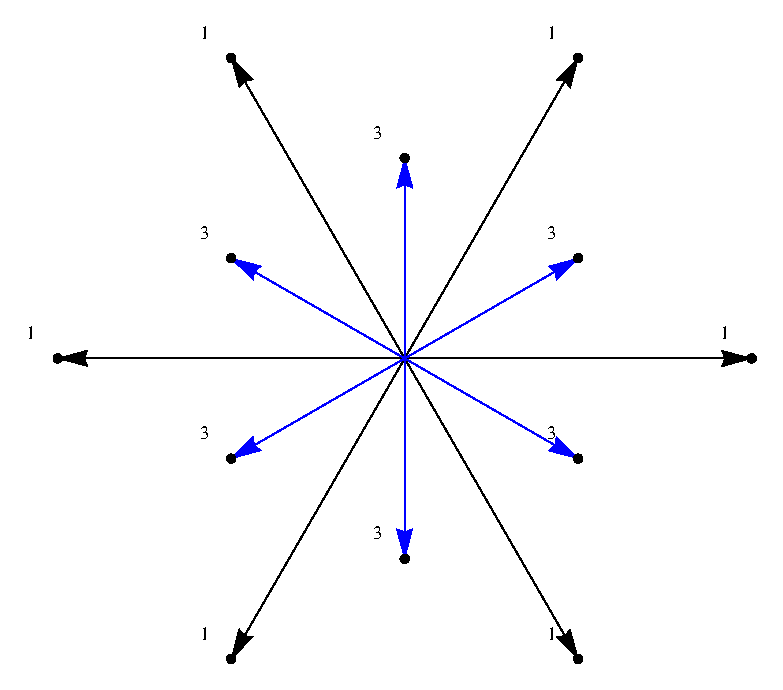
\includegraphics[width=80mm]{Special-A2-D4-all-2}
  }
  \caption{Projection of $D_{4}$ ($so(8)$)-root system onto root space of special subalgebra $A_{2}$
    ($su(3)$). Note that this roots system is $G_{2}$ but with non-trivial multiplicities. }
 \label{fig:d4-a2_splint}
\end{figure}


%% Relying on these theorems we can encode the projections of root system by Dynkin diagrams. We need
%% to allow simple roots to have non-trivial multiplicities. 
%% 

\section{Splints for special embeddings}
\label{sec:splints-spec-embedd}

Since roots are weights of the adjoint representation, such a projection produces the weight diagram
of $\af$-representation that contains adjoint representation of $\af$. After the subtraction of
$\af$-root system $\Delta_{\af}$ from $\Delta'$ we obtain weight diagram of representation called
``characteristic representation of subalgebra $\af$'' by Dynkin in the seminal paper
\cite{dynkin1952semisimple}.

We want to classify all the cases when branching coefficients coincide with weight multiplicities of
some other algebra representations. Such a coincidence is possible when the projection $\Delta'$ of
$\gf$ root system admits a splint $\Delta'=\varphi_{\af}(\Delta_{\af})\cup
\varphi_{\sfr}(\Delta_{\sfr})$, where $\varphi_{\af}$ and $\varphi_{\sfr}$ are the embeddings of
corresponding root systems. The embedding $\varphi_{\af}$ is metric and trivial. Projection of the
root system $\Delta'$ coincides with the projection of weight diagram of the adjoint representation
of algebra $\gf$ with the exception of zero weight. Adjoint representation of $\gf$ contains adjoint
representation of $\af$ and can be decomposed as
\begin{equation}
  \label{eq:3}
  \mathrm{ad}_{\gf}=\mathrm{ad}_{\af}\oplus M_{\af}^{\chi},
\end{equation}
where $M^{\chi}_{\af}$ is not necessary irreducible representation of $\af$ called
``characteristic'' in \cite{dynkin1952semisimple}. 

Weight diagram of $M^{\chi}_{\af}$ coincides with root system $\Delta_{\sfr}$ with the exception of
zero weight. So we need to find all the representations for all simple Lie algebras $\af$, such that
their weight diagrams are root systems after the exclusion of zero weight.

Multiplicity of zero weight in adjoint representation is equal to the rank of the algebra. So if
$\mathrm{rank}\gf-\mathrm{rank}\af$, the representations in questions must be multiplicity-free.

The simplest class of multiplicity-free representations is called ``strongly multiplicity free''
\cite{lehrer2006strongly} and consists of multiplicity free representations with weight systems
admitting strict ordering $\nu_{1}<\nu_{2} \Leftrightarrow \nu_{1}=\nu_{2}+n \alpha$, where $n\in
\mathbb{N}, \alpha\in \Delta^{+}_{\af}$ and for all $\nu_{1},\nu_{2}$ either $\nu_{1}<\nu_{2}$ or
$\nu_{2}<\nu_{1}$.

The list of strongly multiplicity free representations consists of (first) fundamental representations
for series $A_{r}, B_{r}, C_{r}$, exceptional Lie algebra $G_{2}$ (7-dimensional representation) and
all $A_{1}$ representations. 

Fundamental weights of the algebra $A_{r}$ are shorter than its roots, but the projections of $\gf$
weights must be given by linear combinations of roots of special subalgebra $\af$ with integer
coefficients, so the first class of strongly multiplicity free representations does not produce such
projection. 

Nevertheless, the union of diagrams of two fundamental representations of $A_{2}$ with the root
system of $A_{2}$ produces weight diagram of $G_{2}$. This case corresponds to splint
$\Delta_{G_{2}}=\varphi_{1}( \Delta_{A_{2}})\cup \varphi_{2}(\Delta_{A_{2}})$ which is connected
with regular subalgebra $A_{2}\subset G_{2}$ (see Section \ref{sec:splints-root-systems}).


First fundamental representation of $B_{r}$ immediately gives us the splint $\Delta'=\pi_{B_{r}}\left(
\Delta_{D_{r+1}}\right) = \Delta_{B_{r}}\cup \Delta_{A_{1}+\dots+A_{1}}$ corresponding to Gelfand-Tsetlin
multiplicity-free branching for the embedding $so(2r+1)\to so(2r+2)$. 

First fundamental representation of $C_{r}$ -?

Projection $\Delta'$ on the subalgebra $A_{1}$ is never multiplicity free, so $\Delta_{\sfr}$ always
contain parallel roots. The simplest case is special embedding $A_{1}\to A_{2}$ where
$\Delta_{\sfr}$ is the root system $BC_{1}$. Such systems do not correspond to semisimple Lie
algebras, so we can not speak of a coincidence of branching coefficients for the reduction
$\gf\downarrow \af$ with weight multiplicities of $\sfr$-representations. 

Weight diagram of of seven-dimensional representation of $G_{2}$ together with $G_{2}$ root system
form the projection of root system $B_{3}$ which appears in special embedding of simple Lie algebra
$G_{2}\to B_{3}$. Branching coefficients in this case coincide with weight multiplicities of
representations of algebra $\sfr=A_{2}$ with image of root system consisting of short roots of
$G_{2}$. 

The complete classification of multiplicity-free irreducible representations was obtained in
\cite{howe1995perspectives} (see also \cite{stembridge2003multiplicity}).


The weight $\mu$ is minuscule if $\left<\mu,\alpha^{\vee}\right>\leq 1$ for all $\alpha\in
\Delta^{+}$. 

Classification of multiplicity-free irreducible highest weight modules $L^{\mu}$ in
\cite{howe1995perspectives,stembridge2003multiplicity} consists of the following classes:
\begin{itemize}
\item (1) $\mu$ is minuscule,
\item (2) $\mu$ is quasi-minuscule and Lie algebra has only one short simple root,
\item (3) Lie algebra is $sp(6)$ and $\mu=\omega_{1}$, or
\item (4) Lie algebra is $sl(n + 1)$ and  $\mu= m\omega_{1}$ or $\mu  = m\omega_{n}$ 
\end{itemize}

We see that case (1) contains strongly multiplicity free modules of series $A_{r}, B_{r}, C_{r}$ and
exceptional Lie algebra $G_{2}$, strongly multiplicity free modules of $A_{1}$ are included in class
(4). 




What we really need is the classification of all the representations where multiplicities of all
non-zero weights are equal to one. Fortunately, such a classification was obtained in
\cite{plotkin1998visual}. It consists of multiplicity-free representations and adjoint
representations of algebras $B_{r}, C_{r}$ and $F_{4}$. 



(See also https://projecteuclid.org/euclid.jmsj/1180135505 for multiplicity-free branching rules)

Having obtained this classification we need to check which weight diagrams can be obtained as the
projections of $\gf$ root system. It is the case for $B_{n}\to D_{n+1}$ or $A_{1}\oplus\dots\oplus
A_{1}\to D_{n+1}$.



Projection of $\gf$ root system to the root space of $\af$ in many cases can be
encoded by augmented Dynkin diagram with simple root multiplicities not greater or equal than 1.
Number of roots in projection is equal to the number of roots in $\gf$ root system (We do
not consider the case of orthogonal roots here). The rank of augmented Dynkin diagram is the same as
the rank of subalgebra $\af$. Having Lie algebra $\af$ and augmented Dynkin
diagram of the same rank it should be possible to reconstruct the embedding $\af\to
\gf$, though not always in a unique way. 

We must also account for the case of roots of parallel roots of different length. $BC_{1} $ is the
simplest system with parallel roots, one of its two parallel is twice longer than another. Such a
system appear in study of affine 


 The simplest
system with parallel roots have roots of two different length and Such a systems
appear  $BC_{1} $ and its generalization. (We have the dimension of representation of $\af$ and
projection of roots of $\gf$. It's not enough since in general there are different non-equivalent
representations of $\af$. But the number of simple root systems with given number of roots is
finite, so it's possible to check which one has given projection).

Classification of all splints for special embeddings of a given algebra $\af$ is given by
the augmented Dynkin diagrams of the same rank. (!)

Case of diagrams with multiplicities is not particularly interesting since we have just multiple
copies of the same stem (?).


\begin{table}[h]
\begin{tabular}[t]{|p{2em}|p{6em}|p{5em}|p{5em}|p{2em}|p{6em}|}
\hline
Тип & $s$ & $W_a\subset W_s$ & $W_s\subset W_a$ & $g_{inv} $ & Примеры \\
\hline
1 & корневая система & нет & да & есть  & $B_2\rightarrow D_3$, $G_2\rightarrow B_3$\\
\hline
2 & корневая система  & да & да & нет & $A_1\rightarrow A_1+A_1$ \\
\hline
3 & корневая система  & да & нет & есть & $A_1+A_1\rightarrow D_3$ \\
\hline
4 & не корневая система  & да & нет & есть & $A_1\rightarrow A_2$, $A_1\rightarrow B_3$\\
\hline
5 & не корневая система  & да & нет & нет  & $A_1\rightarrow B_2$\\
\hline
6 & \multicolumn{4}{|l|}{$W_a\not\subset W_s$ и $W_s\not\subset W_a$} & $B_2\rightarrow D_4$\\
\hline
\end{tabular}
\caption{Классы специальных сплинтов.}
\label {spsp}
\end{table}


\section*{Conclusion}
\label{sec:conclusion}


\bibliography{special-bibliography}{} 
\bibliographystyle{apalike}
%%  \bibitem{d1}
%%  {\it Е.Б.Дынкин}
%%  Полупростые подалгебры полупростых алгебр.
%%  // Тр. Моск. матем. об-ва, т.1, стр. 39-166 (1952)
%%  \bibitem{d2}
%%  {\it Е.Б.Дынкин}
%%  Максимальные подгруппы классических групп.
%%  // Труды Моск. матем. об-ва, т. 1 (1952)
%%  
%%  
\end{document}
